%!TEX root = sigir2013site_clicks.tex
\section{Background}\label{sec_background}
This section details key works in improving the performance of site search engines by incorporating a variety of different features. This section also provides an overview of works that have utilised clickthrough data for various means.

\begin{figure*}
	\begin{center}
	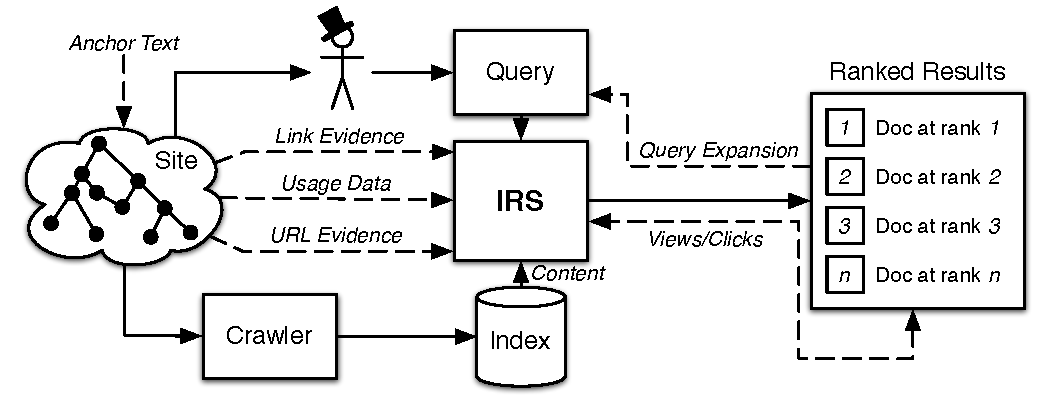
\includegraphics[scale=1.0]{pics/ir_system_new.pdf}
	\end{center}
	\caption{\label{fig:background_architecture}\textbf{A diagram illustrating the basic component architecture of a basic site search system - combined with the different features which have been examined in previous research highlighted in \emph{italics}.\vspace{-0.1cm}}}
\end{figure*}

Today, there are typically three main approaches in which an organisation can deploy site search functionality to their publicly-facing website, intranet, or both. The approaches are:

\begin{itemize}
	
	\item{\textbf{third-party search functionality:} where a commercial Web search engine offers its services for site search;}
	
	\item{\textbf{database driven search:} where an organisation's \emph{Content Management System (CMS)} may provide a SQL-driven search engine, highly unsuitable to semi-structured Web content; and}
	
	\item{\textbf{full-text search engines: } a far superior choice using state-of-the-art technology, with many open-source toolkits in existence for this intent.}
	
\end{itemize}

For the purposes of this paper, we focus exclusively on improving performance of full-text search engines deployed specifically for site search.

\subsection{Improving Site Search}
It is a well recognised problem that the performance of many custom site search engines fall short of the expected standard set by today's modern Web search engines - especially in terms of retrieval accuracy \cite{ding2007log_based_site_search}. Despite the differences in performance, the overall architecture of site search engines are broadly similar to that of a Web search engine - and in turn, a traditional information retrieval system \cite{croft2009search_engine_book}. A diagram depicting the basic architecture of a site search engine can be seen in Figure \ref{fig:background_architecture}, complete with a series of annotations representing features that have been exploited with the aim of improving site search performance. Features examined include: \emph{content}, \emph{link evidence}, \emph{anchor text}, \emph{URL evidence}, \emph{query expansion} and \emph{usage data} (including clickthrough data). It can be noted that many of these techniques have been borrowed from Web search, such are the similarities of the two approaches. In this section, we review research that specifically considers or applies the aforementioned techniques in the context of site search.

Link evidence has been widely exploited by many - if not all - modern Web search engines \cite{upstill2003queryindependent_evidence}, and is considered a powerful approach to improving search performance \cite{carriere1997webquery}. This claim is suitably demonstrated by the \emph{PageRank} algorithm \cite{page1999pagerank}, a cornerstone to Google's success. \citeauthor{carriere1997webquery} \cite{carriere1997webquery} used their \emph{WebQuery} system to examine links amongst documents returned for a given query. The documents with the greatest degree of inlinks were considered ``hot spots'', or documents considered relevant to users. Link evidence was also used by \citeauthor{upstill2003queryindependent_evidence} \cite{upstill2003queryindependent_evidence} in a homepage finding task. Using one enterprise crawl and the TREC WT10G and VLC2 collections, the technique was compared to other forms of query-independent evidence, including \emph{URL-type}, PageRank and anchor text baselines. Their findings showed that more than one form of heuristic should be used in conjunction with link evidence. 

Anchor text has also been examined independently. \citeauthor{fagin2003searching_workplace_web} \cite{fagin2003searching_workplace_web} conducted a study on the IBM intranet where several heuristics were used. Those included were PageRank, inlinks, crawl dates and URL evidence. The use of PageRank and anchor text were considered ``extremely valuable for intranet search'', improving the quality of results returned. They also found the intranet to be jargon-heavy, with users unaware of this. The authors hypothesised that such an issue would hold across other intranets. \citeauthor{upstill2003queryindependent_evidence} \cite{upstill2003queryindependent_evidence} reiterated the findings of \citeauthor{fagin2003searching_workplace_web} \cite{fagin2003searching_workplace_web}, determining that PageRank and anchor text in combination provided an improvement to site search, but may not have been satisfactory by themselves. \citeauthor{hawking2004link_site_search} \cite{hawking2004link_site_search} complemented these findings. While they found improvements in retrieval performance when utilising anchor text from within an organisation's website/intranet, anchor text from external sources was found to be superfluous to improving performance. This finding was used as part of the study by \citeauthor{ding2007log_based_site_search} \cite{ding2007log_based_site_search}, who disregarded any evidence from external documents for the site they were examining. However, \citeauthor{upstill2003queryindependent_evidence} \cite{upstill2003queryindependent_evidence} claim that utilising anchor text from external sources would complement site search due to the smaller collection of documents websites possess compared to the larger Web.

Usage data - in the form of server logs - has been also exploited by many, with server logs described by \citeauthor{guo2009click_chain} \cite{guo2009click_chain} as a ``gold mine'' of information. Such information can be used to help augment site search performance \cite{ding2007log_based_site_search}, and are under the ownership of a website's owner, removing any legal or financial barriers for access \cite{cui2005web_logs_site_search}. \citeauthor{xue2002log_mining} \cite{xue2002log_mining} used server log analysis to improve performance through use of generalisation rule mining. This approach included a hierarchical taxonomy of a given website. The authors then reranked documents by incorporating the taxonomy and prior user behaviours to yield a 15\% improvement over an unspecified ``full-text search'' approach. \citeauthor{cui2005web_logs_site_search} \cite{cui2005web_logs_site_search} constructed a probabilistic graph from log analysis and calculated a new score, \emph{LPageRank}, from webpages within Eastern Kentucky University's domain. The score combined traditional PageRank with other factors, such as the previous number of visits and traffic access patterns. Their results outperformed a traditional PageRank baseline. Finally, \citeauthor{ding2007log_based_site_search} \cite{ding2007log_based_site_search} improved site search performance using a novel approach consisting of two separate indexes. A content-based index, extracted from URLs in server logs, was combined with an anchor-based index. Results showed a maximum performance increase of 22.8\%.

Query expansion has been used by \citeauthor{albakour2012query_reformulations_local} \cite{albakour2012query_reformulations_local}, who performed a study examining query reformulations from a university website. Analysis of query logs showed users were successfully able to reformulate their queries. Clickthrough data was also used as a metric to help identify useful query reformulations. \citeauthor{kruchwitz2013query_suggestions} \cite{kruchwitz2013query_suggestions} also recently conducted a study on different query modification techniques with data collected from site search logs. They found that clustering queries together based upon individual search sessions commonly produced relevant query suggestions.

\subsection{Clickthrough Data - Uses and Issues}\label{sec:background_clickthrough}
Clickthrough data has been exploited for a variety of different purposes. As a form of \emph{implicit relevance feedback}, clickthrough data can be theoretically generated in unlimited volumes \cite{joachims2002optimizing_clickthrough}, but is subject to adverse qualities such as noise and bias \cite{kelly2004time_implicit}. Despite this, clickthrough data is still regarded as a reliable form of implicit feedback \cite{joachims2005clickthrough} and is easy to collect in a non-laboratory setting.

\citeauthor{joachims2005clickthrough} \cite{joachims2005clickthrough} conducted a user study investigating the reliability of clickthrough data as a form of implicit feedback. Two types of analysis were conducted. Eyetracking was recorded to examine how users interacted with a Google results page, the findings of which were compared against \emph{explicit relevance judgements}. Results showed relative preferences were ``reasonably accurate on average'', but also showed a user's clicking habits were intrinsically biased in two ways. \emph{Positional bias} showed that users trusted the retrieval method used by only clicking on documents high in the rankings. This behaviour was also observed by \citeauthor{granka2004eyetracking} \cite{granka2004eyetracking}. A \emph{quality bias} also showed that clicking behaviour was not only influenced by the relevance of a clicked link, but also by the overall quality of the other abstracts for surrounding documents.

Many techniques used to evaluate the reliability of clickthrough data use explicit relevance judgements, or \emph{editorial judgements}. However, an organisation wishing to improve their site search offering would likely not be able to afford or attain such judgements for their documents. \citeauthor{dupret2010intrinsic_document_relevance_clickthrough_logs} \cite{dupret2010intrinsic_document_relevance_clickthrough_logs} devised the \emph{Cumulative Relevance Model}, based upon explicit assumptions of a user's behaviour. These assumptions accounted for his or her actions throughout a search session, which was considered successful if it ended with a click on a ranked document. The model proved useful for sessions with low click rates - an inherent problem of site search. \citeauthor{hofmann2011graded_relevance} \cite{hofmann2011graded_relevance} showed how judgements obtained from clickthrough data could be evaluated.

Studies have also focused on how clickthrough data can improve search performance, such as those by \citeauthor{agichtein2006improving_web_search} \cite{agichtein2006improving_web_search} and \citeauthor{xue2003web_logs_site_search} \cite{xue2003web_logs_site_search}. In \cite{agichtein2006improving_web_search}, clickthrough data was incorporated using a machine-learned function, and was demonstrated to outperform competitive Web search ranking algorithms by as much as 31\%.